\normaltrue \difficilefalse \tdifficilefalse
\correctiontrue

%\UPSTIidClasse{11} % 11 sup, 12 spé
%\newcommand{\UPSTIidClasse}{12}

\exer{Mouvement RR 3D  $\star$ \label{B2:13:07:02}}
\setcounter{question}{0}\marginnote{\UPSTIcompetence{B2-13}}
\index{Compétence B2-13}
\index{Mécanisme à 2 rotations 3D}
\ifcorrection
\else
\marginnote{\textbf{Pas de corrigé pour cet exercice.}}
\fi

\ifprof
\else
Soit le mécanisme suivant. On a $\vect{AB}=R\vect{i_1}$ et $\vect{BC}=\ell\vect{i_2}+r\vect{j_2}$. On note $R+\ell=L = \SI{20}{mm}$ et $r=\SI{10}{mm}$.
\begin{center}
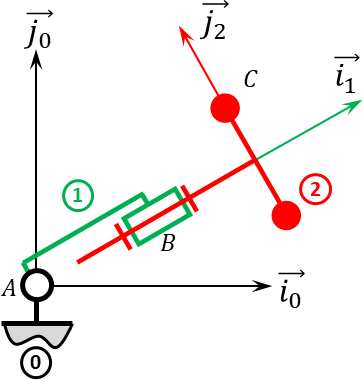
\includegraphics[width=.8\linewidth]{07_RR3D_01}
\end{center}
\fi

%=====================================
\ifprof
\else
\ifcolle
\else
\marginnote{
\begin{solution}
\begin{enumerate}
\item $\vectv{C}{2}{0}= \left(R+\ell\right)\dot{\theta}\vj{1} -r\dot{\theta}\cos\varphi \vi{1} + r\dot{\varphi}\vk{2}$.
\item  $\vectv{C}{2}{0}=r\dot{\varphi}\vk{2}-r\dot{\theta}\cos\varphi\vi{1}+\ell\dot{\theta}\vj{1}+R\dot{\theta}\vj{1}$.
\item $\torseurcin{V}{2}{0} = \torseurl{\dot{\theta}\vk{1}+ \dot{\varphi}\vi{1}}{\left(R+\ell\right)\dot{\theta}\vj{1} -r\dot{\theta}\cos\varphi \vi{1} + r\dot{\varphi}\vk{2}}{C}$.
\item $\vectg{C}{2}{0} =\left(R+\ell\right)\ddot{\theta}\vj{1} -\left(R+\ell\right)\dot{\theta}^2\vi{1} 
-r\ddot{\theta}\cos\varphi \vi{1} +r\dot{\theta}\dot{\varphi}\sin\varphi \vi{1} -r\dot{\theta}^2\cos\varphi \vj{1} 
+ r\ddot{\varphi}\vk{2}+ r\dot{\varphi}\left(\dot{\theta}\sin\varphi\vi{1}- \dot{\varphi}\vj{2} \right)$.
\end{enumerate} 
\end{solution}}
\fi
\marginnote{Corrigé voir \ref{B2:13:07}.}
\fi
%=====================================


\question{Déterminer $\vectv{C}{2}{0}$ par dérivation vectorielle.}
\ifprof ~\\
$\vectv{C}{2}{0}$ 
$=\deriv{\vect{AC}}{\rep{0}}$ 
$=\deriv{R\vi{1}+\ell\vi{2}+r\vj{2}}{\rep{0}}$.

Calculons : 
\begin{itemize}
\item $\deriv{\vi{1}}{\rep{0}}$ $=\vecto{1}{0} \wedge \vi{1}$ $=\dot{\theta}\vk{0} \wedge \vi{1}$ $=\dot{\theta}\vj{1}$.
\item $\deriv{\vi{2}}{\rep{0}}$ $=\dot{\theta}\vj{1}$ ($\vi{1}=\vi{2}$).
\item $\deriv{\vj{2}}{\rep{0}}$ $=\vecto{2}{0} \wedge \vj{2}$ 
$=\left(\dot{\theta}\vk{0}+ \dot{\varphi}\vi{1} \right) \wedge \vj{2}$
$=\dot{\theta}\vk{1} \wedge \vj{2}+ \dot{\varphi}\vi{1}  \wedge \vj{2}$
$=-\dot{\theta}\cos\varphi \vi{1} + \dot{\varphi}\vk{2} $.
\end{itemize}

On a donc, 
$\vectv{C}{2}{0}= \left(R+\ell\right)\dot{\theta}\vj{1} -r\dot{\theta}\cos\varphi \vi{1} + r\dot{\varphi}\vk{2}$.
\else
\fi


\question{Déterminer $\vectv{C}{2}{0}$ par composition.}
\ifprof ~\\
On a $\vectv{C}{2}{0}= \vectv{C}{2}{1}+\vectv{C}{1}{0}$.
\begin{itemize}
\item $\vectv{C}{2}{1}$ : on passe par $B$ car $B$ est le centre de la pivot entre 2 et 1 et que $\vectv{B}{2}{1}=\vect{0}$. 
$\babarv{C}{B}{2}{1} =\left(-\ell\vi{2}-r\vj{2} \right)\wedge \dot{\varphi}\vi{1} $ 

$=-\ell\vi{2}\wedge \dot{\varphi}\vi{1}-r\vj{2} \wedge \dot{\varphi}\vi{1}$.

$=r\dot{\varphi}\vk{2}$.

\item $\vectv{C}{1}{0}$ : on passe par $A$ car $A$ est le centre de la pivot entre 1 et 0 et que $\vectv{A}{1}{0}=\vect{0}$ est nul. 
$\babarv{C}{A}{1}{0}$ 

$=\left(-r\vj{2}-\ell\vi{2}-R\vi{1}\right)\wedge \dot{\theta}\vk{1}$

$=-r\dot{\theta}\cos\varphi\vi{1}+\ell\dot{\theta}\vj{1}+R\dot{\theta}\vj{1}$ %%
\end{itemize}

Au final, 
 $\vectv{C}{2}{0}=r\dot{\varphi}\vk{2}-r\dot{\theta}\cos\varphi\vi{1}+\ell\dot{\theta}\vj{1}+R\dot{\theta}\vj{1}$.
\else
\fi


\question{Donner le torseur cinématique $\torseurcin{V}{2}{0}$ au point $C$.}
\ifprof ~\\
$\torseurcin{V}{2}{0} = \torseurl{\dot{\theta}\vk{1}+ \dot{\varphi}\vi{1}}{\left(R+\ell\right)\dot{\theta}\vj{1} -r\dot{\theta}\cos\varphi \vi{1} + r\dot{\varphi}\vk{2}}{C}$
\else
\fi

\question{Déterminer $\vectg{C}{2}{0}$.}
\ifprof ~\\
 
 $\vectg{C}{2}{0} = \deriv{\vectv{C}{2}{0}}{\rep{0}}$
 
 $ = \deriv{\left(R+\ell\right)\dot{\theta}\vj{1} -r\dot{\theta}\cos\varphi \vi{1} + r\dot{\varphi}\vk{2}}{\rep{0}}$
 
 Calculons : 
\begin{itemize}
\item $\deriv{\vi{1}}{\rep{0}}$ $=\vecto{1}{0} \wedge \vi{1}$ $=\dot{\theta}\vk{0} \wedge \vi{1}$ $=\dot{\theta}\vj{1}$.
\item $\deriv{\vj{1}}{\rep{0}}$ $=\vecto{1}{0} \wedge \vj{1}$ $=\dot{\theta}\vk{0} \wedge \vj{1}$ $=-\dot{\theta}\vi{1}$.
\item $\deriv{\vk{2}}{\rep{0}}$ $=\vecto{2}{0} \wedge \vk{2}$ 
$=\left(\dot{\theta}\vk{0}+ \dot{\varphi}\vi{1} \right) \wedge \vk{2}$
$=\dot{\theta}\vk{1} \wedge \vk{2}+ \dot{\varphi}\vi{2}  \wedge \vk{2}$
$=\dot{\theta}\sin\varphi\vi{1}- \dot{\varphi}\vj{2}$.
\end{itemize}

$\vectg{C}{2}{0}$ 
$ =\left(R+\ell\right)\ddot{\theta}\vj{1} -\left(R+\ell\right)\dot{\theta}^2\vi{1} 
-r\ddot{\theta}\cos\varphi \vi{1} +r\dot{\theta}\dot{\varphi}\sin\varphi \vi{1} -r\dot{\theta}^2\cos\varphi \vj{1} 
+ r\ddot{\varphi}\vk{2}+ r\dot{\varphi}\left(\dot{\theta}\sin\varphi\vi{1}- \dot{\varphi}\vj{2} \right)$.
\else
\fi

